\documentclass[12pt]{report}

\usepackage{url}
\usepackage[utf8]{inputenc}
\usepackage[english,russian]{babel}
% \usepackage{tocvsec2}

\usepackage[dvips]{graphicx}
\graphicspath{{images/}}

\usepackage{tikz}
\usepackage{listings}
\usepackage{subfigure}

\renewcommand{\rmdefault}{ftm}
\usepackage[T2A]{fontenc}
\usepackage{setspace}
\setstretch{1.5}

\usepackage{geometry}
\geometry{top=2cm}
\geometry{bottom=2cm}
\geometry{left=3cm}
\geometry{right=1.5cm}

\renewcommand\contentsname{Содержание}
% \setcounter{tocdepth}{2}

\renewcommand{\baselinestretch}{1.5}
\usepackage{indentfirst}

\begin{document}
	
	{\thispagestyle{empty}
		\begin{center}
			\scriptsize Министерство образования и науки Российской Федерации\\
			\scriptsize Федеральное государственное автономное образовательное учреждение высшего образования\\
			\normalsize\bf <<Уральский федеральный университет\\
			\normalsize\bf имени первого Президента России Б.Н. Ельцина>>
		\end{center}
		
		\begin{center}
			\normalsize\bf Институт естественных наук и математики\\
			\normalsize\bf Департамент математики, механики и компьютерных наук\\
		\end{center}
		
		\vspace{3cm}
		
		\begin{center}
			\LARGE\bf Исследование потокобезопасных неблокирующих структур данных
		\end{center}
		
		\vspace{2.5cm}
		
		\hspace{-1cm}
		\begin{minipage}{80mm}
			\noindent
			\vspace{-2.3cm}
			\begin{flushleft}
				\begin{spacing}{1.0}
					\large <<Допущен к защите>>\\
					\hspace{6cm}\\
					\large Директор департамента\\
					\large к.ф.-м.н., доцент\\
					\large Асанов~М.~О.
					\underline{\hspace{6cm}}\\
					<<\underline{\hspace{0.7cm}}>>\underline{\hspace{3cm}}2017 г.
				\end{spacing}
			\end{flushleft}
		\end{minipage}
		\begin{minipage}{90mm}
			\begin{flushleft}
				\begin{spacing}{1.0}
					\large Квалификационная работа на соискание степени бакалавра наук по направлению\\
					\large <<Фундаментальная информатика и информационные технологии>>\\
					\large студента группы ФТ-401 (МЕН-430802) Сваловой~А.~А.\\
					\large Научный руководитель:\\
					\large Ассистент департамента\\
					\large Плинер~Ю.~А.
				\end{spacing}
			\end{flushleft}
		\end{minipage}
		
		\vfill
		
		\begin{center}
			Екатеринбург\\
			2017 год
		\end{center}
	}
	
	\newpage
	
	{\pagestyle{plain}
		\tableofcontents
	}
	
	\newpage
	
	\chapter*{Реферат}
	\addcontentsline{toc}{chapter}{Реферат}
	
		\par Свалова~А.~А. ИССЛЕДОВАНИЕ ПОТОКОБЕЗОПАСНЫХ НЕБЛОКИРУЮЩИХ СТРУКТУР ДАННЫХ, квалификационная работа: стр. 23, табл 1.
		\par Ключевые слова: Многопоточность, структуры данных, Блокирующие и неблокирующие алгоритмы.
		\par В данной работе описаны некоторые потокобезопасные неблокирующие структуры данных. Для этих структур данных приведены сценарии и результаты тестирования.
	
	\newpage
	
	{\pagestyle{plain}
		
		\chapter*{Введение}
		\addcontentsline{toc}{chapter}{Введение}
		
		\large Технический прогресс в области электронных устройств привёл к появлению многоядерных процессоров и многопроцессорных систем. Одной из основных задач программистов стало написание программ, способных эффективно использовать эту особенность и выполняться на нескольких ядрах и процессорах. В наше время всё чаще возникает потребность в использовании специальных алгоритмов и структур данных для этого. Последним и посвящена эта работа.
		
		\textit{Процессом} называется последовательное выполнение инструкций заданной программы \cite{Tanenb}. 
		
		\textit{Многопоточностью} называют определённое свойство процесса операционной системы. Многопочтоный процесс может состоять из нескольких потоков, выполняющихся <<параллельно>>, то есть без предписанного порядка \cite{Tanenb}. 
		
		\textit{Поток выполнения} или поток~--- это подпроцесс, выполняющийся в контексте полноценного процесса. Потоки одного процесса работают параллельно, не зависимо друг от друга, но могут синхронизировать свою работу при необходимости. \cite{Tanenb}.
		
		В общем случае использование многопоточности помогает ускорять выполнение вычислительных задач. Однако за это приходится платить проблемами, связанными с доступом к общим ресурсам (например, памяти) из разных потоков. Во всех современных операционных системах потоки одного процесса могут иметь доступ к общей памяти, что позволяет им обмениваться данными.
		
		Если несколько потоков одновременно захотят изменить общую память, может возникнуть одна из ошибок параллельного программирования: потерянное обновление, грязное чтение, неповторяющееся чтение, чтение фантомов или состояние гонки \cite{wikiRace}.
		В качестве примера можно рассмотреть следующий процесс: два потока хотят прибавить единицу к некоторой общей переменной. Они считывают значение переменной в локальную память, прибавляют единицу к полученному значению и по очереди в случайном порядке перезаписывают значение в общей памяти на значение из локальной памяти. В итоге переменная увеличивается только на единицу, а не на двойку, как ожидалось.
		
		Чтобы разрешить эту проблему, необходимо разделение доступа к общей памяти и другим разделяемым ресурсам. 
		
		\textit{Синхронизация потоков}~--- это механизм, позволяющий обеспечить корректную работу из нескольких потоков с~общим ресурсом при условии, что доступ к нему может потребоваться в~случайном порядке \cite{Sync}. Общим ресурсом может выступать файл на файловой системе, общая память, открытый сокет и т.~д.
		
		Синхронизацию можно реализовать несколькими способами, но самым простым из них является \textit{блокировка}. Каждый раз, когда поток хочет осуществить операцию с ресурсом, он блокирует этот ресурс. В любой момент времени только один птоок может владеть блокировкой заданного ресурса. После окончания работы с ресурсом блокировка снимается. Если другому потоку нужен доступ к общему ресурсу, защищённому блокировкой, то выполнение этого поток останавливается до тех пор, пока блокировка не будет снята. \cite{lockmsdn}.
		
		Основное преимущество блокировки как механизма синхронизации заключается в его простоте. Большинство современных операционных систем содержат низкроуровневую реализацию блокировок~--- мьютексы и семафоры \cite{Tanenb}. Благодаря этому в арсенале программиста оказывается простой и мощный инструмент для организации блокировок.
		
		Однако у блокировок есть и минусы:
		
		\begin{itemize}
			\item если одновременно много потоков хотят получить доступ к общему ресурсу, то в процессе возникает <<узкое горлышко>>~--- все потоки ожидают снятия блокировки, а выполнение процесса практически полностью приостанавливается \cite{mutex};
			\item если внутри блокировки выполняется достаточно большой участок программы, теряется основной смысл многопоточности. Внутри таких участков в каждый момент времени может находиться только один поток, а мы теряем преимущества многопоточности, когда, например, одна и та же задача для разных объектов может выполняться одновременно;
			\item возможна ситуации, когда поток захватил ресурс A и ждет освобождение ресурса B, в то время как второй поток захватил ресурс B и ждет освобождения ресурса A. Такая ситуация называется взаимной блокировкой (англ. deadlock \cite{deadlock}, \cite{deadlock2}). Программа  останавливает свое выполнение и не может разрешить эту ситуацию без вмешательства извне.
		\end{itemize}
		
		Наличие недостатков блокировок привели исследователей к необходимости создания других методов синхронизации. Одним из них является неблокирующая синхронизация. 
		
		\textit{Неблокирующая синхронизация} это метод синхронизации, в котором потоки не могут используть блокировки.
		
		Синхронизация при этом обычно осуществлется с помощью специальных аппаратно-поддерживаемых атомарных операций \cite{introLockFree}. Примером такой операции является \textit{Compare-And-Change} от трёх аргументов $x$, $y$ и $z$. Она сравнивает $x$ с $y$ и если они равны, то выполняет присваивание $x := z$. Процессором гарантируется, что эта операция будет выполнена атомарно, то есть между сравнением и присваиванием не может быть выполнена никакая другая операция. Поток может узнать, выполнилось ли присваивание в операции \textit{Compare-And-Change}. Именно это свойство позволяет строить работающие неблокирующие синхронизации. Подробнее об атомарных операциях рассказывается в первой главе.			
		
		Область исследования неблокирующих алгоритмов является активно развивающейся, так как не всегда можно достаточно просто переписать блокирующую версию многопоточного алгоритма так, чтобы вместо блокировок использовать только неблокирующие атомарные операции. Для некоторых даже простых структур данных до сих пор не придуманы неблокирующие способы реализации. Примером такой структуры данных является обычный массив.
		
		Однако задача придумывания неблокирующих алгоритмов имеет под самой практическую значимость: часто они оказываются быстрее блокирующих аналогов. Правда, на практике это нередко зависит от деталей реализации, области применение и др.
		
		\textbf{Объектом исследования} данной работы являются неблокирующие алгоритмы для работы со структурами данных. Они описаны во второй главе этой работы.
		
		Цели работы:
		\begin{itemize}
			\item изучить неблокирующие алгоритмы, реализующие интерфейс, включающий добавление элемента в множество, удаление и проверку на принадлежность к множеству;		\item адаптировать алгоритмы, разработанные под языки программирования с неуправляемой памятью, к языкам с управляемой памятью;
			\item реализовать эти алгоритмы C\#;
			\item проверить с помощью тестов производительности, являются ли рассмотренные неблокирующие алгоритмы эффективнее аналогичных блокирующих.
		\end{itemize}
		
		Для сравнения были выбраны следующие структуры данных, реализующие описанный выше функционал множества: сортирующийся лист, хеш-таблица, список с пропусками и самобалансирующееся дерево поиска. Для сравнения неблокирующих реализаций с блокирующими взяты реализации этих же структур данных из стандартной библиотеки .NET. О методиках тестировании и его результатах рассказывается в третьей главе.			
		
		В открытом репозитории GitHub \cite{My} приведены результаты сравнений этих структур данных и разные варианты использования их на практике.			
		
		\chapter{Общие сведения}
		
		\section{Классификация алгоритмов и атомарная операция}
		
		Неблокирующие алгоритмы традиционно можно разделить на три класса: Wait-free, Lock-free и Obstruction-free алгоритмы \cite{WaitFree}.
		
		В Wait-free алгоритмах каждый поток совершает операции за конечное число шагов вне зависимости от других потоков. Данное ограничение является очень сильным, поэтому, к сожалению, редко достигается.
		
		В Lock-free алгоритмах конкретный поток может остановиться, но гарантируется, что система в целом двигается вперёд. Если какой-то поток не смог выполнить операцию, значит, что какой-то другой поток смог выполнить свою операцию, следовательно, в целом система продвинулась.
		
		В третьем типе каждый может выполнить каждую операцию за конечное количество шагов, если ничего ему не помешает. В данном случае может случиться ситуация, когда ни один из потоков не двигается вперед, однако ни один заблокированный поток не может мешать работе всех остальных потоков, следовательно, это все равно более сильная гарантия, чем блокирущие алгоритмы.
		
		Это самое сильное требование из-за чего редко реализуемое, однако существует алгоритм, преобразующий Obstruction-free в Wait-free \cite{waitFree2}
		
		Каждая из этих реализаций использует абстракцию <<атомарная операция>> - это операция, которая либо не выполняется совсем, либо выполняется как единое целое. В данной работе используется атомарная операция Compare~And~Swap~(CAS) (Рис~\ref{pic:CAS}). Эта операция сравнивает две ссылки и, если они равны, меняет одну из них на новую. Эта операция предоставляется большинством операционных систем и уже встроена в язык C\#.
		\begin{figure}[h]
			\begin{lstlisting}
	CAS(ref reference, newReference, comparand)
			\end{lstlisting}
			\caption{CAS сравнивает reference с comparand и, если они равны, заменяет reference на newReference}
			\label{pic:CAS}
		\end{figure}
		
		\section{Известные алгоритмы и их особенности}
		
		Первой структурой данных, для которой был создан неблокирующий алгоритм вставки, удаления и проверки на принадлежность, был стек. Первое упоминание потокобезопасных неблокирующих структур данных было описано в статье Трейбера в 1986 году \cite{Treiber}. Это самый простой и самый известный алгоритм на данный момент. В данном алгоритме может возникнуть ситуация, когда большое количество потоков единовременно пытается изменить один и тот же ресурс. Тогда каждый поток в цикле будет пробовать атомарно изменить ресурс и при успешной попытке выходить из цикла. Чтобы уменьшить количество таких попыток используется стратегия Back-off - стратегия, при которой в случае неуспешной попытки применения атомарной операции поток на какое-то время засыпает или пытается сделать какую-то другую полезную работу, а потом снова пытается повторить атомарную операцию. Это позволяет уменьшить давление на критические данные контейнера при большой нагрузке. Данная стратегия очень часто встречается в неблокирующих алгоритмах. Количество времени, на которое нужно заснуть, а так же выбор полезной работы выбирается в каждом конкретном случае индивидуально.
		
		Другой не менее известный алгоритм - алгоритм очереди, описанный в статье Михаеля и Скотта в 1996 году \cite{Queqe}. В нем для поддержания двух ссылок на <<голову>> и на <<хвост>> используется еще одна популярная стратегия - вставка ложного (sentinel) элемента специальной структуры, который не хранит в себе никакого значения, а нужен исключительно для удобства использования и более простого описания алгоритма.
		
		В двухтысячных годах тема стала популярной и начали появляться улучшения этих алгоритмов, а также создаваться новые алгоритмы других структур данных, таких как: списки\cite{LinkedList}, списки с пропусками \cite{ListSkipList},  хеш-таблицы \cite{HashTable}, некоторые деревья и др. Однако не все структуры данных можно реализовать неблокирующими. В таких случаях используют подход, объединяющий блокирующий и неблокирующий. Блокировка захватывается только на отдельные небольшие участки памяти, независимо друг от друга. В таких алгоритмах особо часто используемые операции производятся без блокировок, а некоторые операции производятся с блокировками, но на маленькие участки памяти. Такие алгоритмы оказываются проще в понимании и доказательстве, но не проигрывают в эффективности и применимости.  
		
		Один из способов такой локальной блокировки - это добавление особого маркера в ссылку на объект. Так, если один поток смог атомарно изменить ссылку на некоторый объект, пометив ее этим маркером, все остальные потоки понимают, что данный объект используется в какой-то операции и его нельзя изменять. 
		
		В языках с неуправляемой памятью такой способ легко осуществим благодаря выравниванию указателей на объект. При выделении памяти компилятор, обычно, выравнивает длину указателя на максимально большой тип данных. Поэтому в указателе остаются реально неиспользуемые биты, которые можно как раз и использовать в качестве маркера.
		
		В языках с управляемой памятью разработчик не имеет доступа к ссылке, поэтому стоит придумывать способы сымитировать эту ссылку с помощью объектов. В данной работе реализован примитив маркируемой ссылки (Atomic Markable Reference). Он будет хранить в себе текущее состояние этой ссылки (Рис~\ref{pic:AMR}). Само же состояние будет состоять из непосредственно ссылки и описанного выше маркера. В данном случае маркер как раз отвечает за неиспользуемые биты указателя. Теперь можно атомарно изменять ссылку на состояние, что равносильно изменению помеченного указателя. Изменяя этот примитив, можно сымитировать изменение указателя, что позволяет также использовать алгоритмы с локальными блокировками. 		
		\begin{figure}[h]
			\begin{lstlisting}
	public class AtomicMarkableReference<TReference, TMark>
	{
		volatile State state;
		
		private class State
		{
			TReference Reference;
			TMark Mark;
		}
	}
			\end{lstlisting}
			\caption{AtomicMarkableReference}
			\label{pic:AMR}
		\end{figure}
		
		\section{Проблема ABA}
		
		При неправильной организации кода в неблокирующих алгоритмах могут возникнуть проблемы. Самая известная~--- проблема ABA \cite{ABA}. Эта проблема возникает, когда множество потоков обращаются к разделяемой памяти поочерёдно. Алгоритм может рассчитывать, что если атомарная операция завершилась успехом - значит память не менялась. Но CAS всего лишь гарантирует, что ее значение в момент, когда он ее перезаписал, было равно тому значению, которое ему передано как ожидаемое. Если из списка удалить элемент, уничтожить его, а затем создать новый элемент и добавить обратно в список, есть вероятность, что новый элемент будет размещён на месте старого. Указатель на новый элемент совпадёт с указателем на старый, что и приведёт к проблеме. Такая проблема может возникнуть только в языках программирования с неуправляемой памятью. В языках программирования с управляемой памятью существует абстракция <<сборщик мусора>>, которая обеспечивает отсутствие потери и повторного использования ссылок.
		
		\section{Set}
		
		Set~--- это коллекция для хранения неупорядоченного множества уникальных объектов. Это аналог математического понятия \textit{множество} Эта структура данных позволяет добавлять элементы, удалять элементы и быстро проверять, существует ли уже такой элемент (Рис~\ref{pic:Set}). 
		\begin{figure}[h]
			\begin{lstlisting}
public interface ISet<TElement>
{
	bool Add(TElement element);
	bool Contains(TElement element);
	bool Remove(TElement element);
}
			\end{lstlisting}
			\caption{Интерфейс ISet}
			\label{pic:Set}
		\end{figure}
		\par Чаще всего set применяют для объединения объектов с какими-то общими свойствами. Эта структура данных близка к map, которая используется повсеместно. Пример: индексы в базах данных.
		\par Хотя операции в set могут быть реализованы произвольным способом, но чаще всего его используют для быстрой проверки принадлежности элемента (черные, белые списки, базы данных). Поэтому в данной работе будет сделан акцент на быстром поиске. Быстрое добавление тоже будет играть роль, поэтому придется пожертвовать скоростью удаления.		
		
		\chapter{Реализации алгоритмов}
		\par В данной главе будут приведены краткие описания неблокирующих алгоритмов, проблемы, которые они решают и сложности реализации. Полное описание алгоритмов можно найти в списке литературы \cite{LinkedList}, \cite{ListSkipList}, \cite{ListAndSkipList}, \cite{HashTable}, \cite{artOfMultiprocessor}. Стандартные реализации однопоточных алгоритмов общедоступны, поэтому не будут описаны в данной работе. Познакомиться с ними можно, например, в книге <<Структуры данных и алгоритмы>> \cite{dataStructures}.
		\section{Односвязный список}
		\par Пусть односвязный список состоит из элементов, в каждом из которых есть значение этого элемента и ссылка на следующий элемент (Рис~\ref{pic:listNode}). Поиск элемента не будет рассмотрен, так как он совпадает с поиском в обычном сортирующимся списке.
		\begin{figure}[h]
			\begin{lstlisting}
public class LinkedListNode<TElement>
{
	TElement Element;
	LinkedListNode<TElement> Next;
}
			\end{lstlisting}
			\caption{Вершина списка}
			\label{pic:listNode}
		\end{figure}
		\par Если реализовать добавление как в однопоточном варианте, то возможна проблема при одновременном добавлении двух последовательных элементов. Пусть, есть список с элементами \textbf{1}-\textbf{2}-\textbf{5} (Рис~\ref{pic:doubleInsertA}). Поток \textbf{А} хочет вставить элемент \textbf{3}, поток \textbf{Б} - элемент \textbf{4}. Поток А понимает, что ему нужно вставить элемент между \textbf{2} и \textbf{5}. Он запоминает ссылку на предыдущий и следующий элементы и в этот момент операционная система передает управление потоку \textbf{Б} (Рис~\ref{pic:doubleInsertB}). Поток \textbf{Б} также находит место для вставки и тоже запоминает \textbf{2}, как предыдущий элемент, \textbf{5}, как следующий (Рис~\ref{pic:doubleInsertC}). После этого он переписывает ссылку <<Следующий>> у элемента \textbf{2} на новосозданный элемент \textbf{4}, а у элемента \textbf{4} на \textbf{5} (Рис~\ref{pic:doubleInsertD}). Управление возвращается к потоку \textbf{А}. Он перезаписывает ссылку <<Next>> предыдущего элемента \textbf{(2)} на новосозданный элемент \textbf{3}, а ссылку элемента \textbf{3} на следующий элемент \textbf{(5)} (Рис~\ref{pic:doubleInsertE}). В результате элемент \textbf{4} <<потеряется>>, т. е. не будет ни одной ссылки, указывающей на него.
		\begin{figure}[h!]
			\begin{minipage}[h]{0.45\linewidth}
				\center \subfigure[]{
					{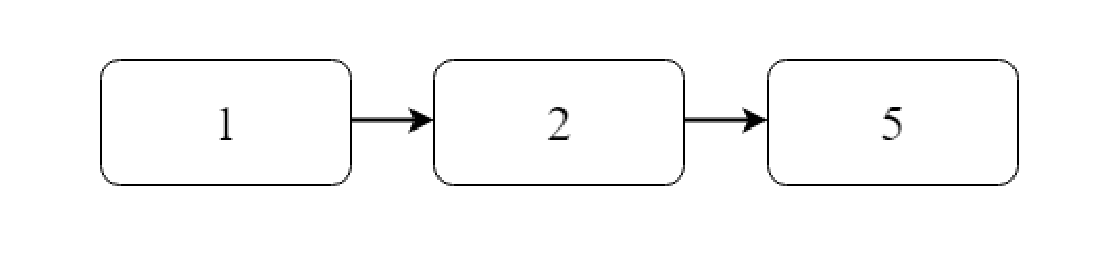
\includegraphics[width=1\linewidth]{1}}
					\label{pic:doubleInsertA}
				}
			\end{minipage}
			\hfill
			\begin{minipage}[h]{0.45\linewidth}
				\center \subfigure[]{
					{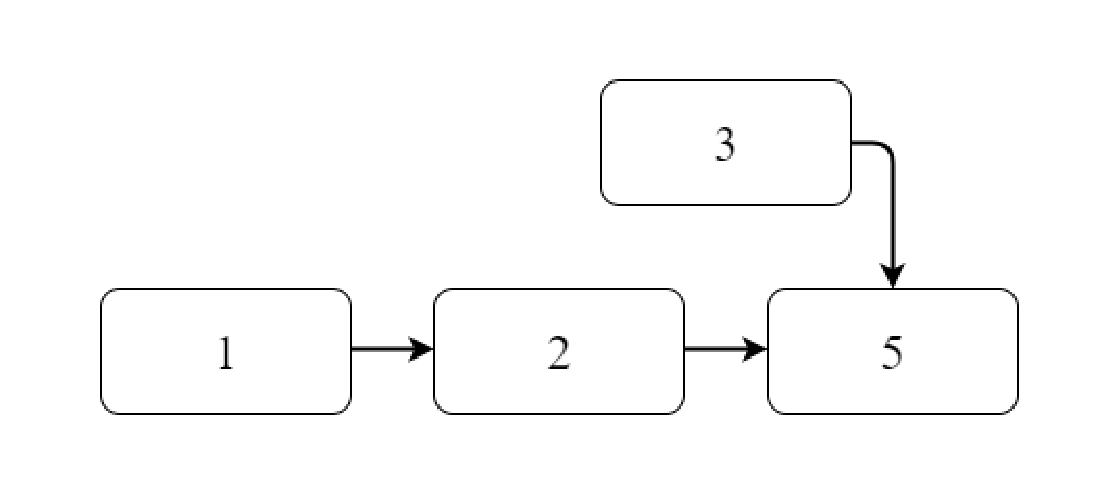
\includegraphics[width=1\linewidth]{2}}
					\label{pic:doubleInsertB}
				}
			\end{minipage}
			\vfill
			\begin{minipage}[h]{0.45\linewidth}
				\center \subfigure[]{
					{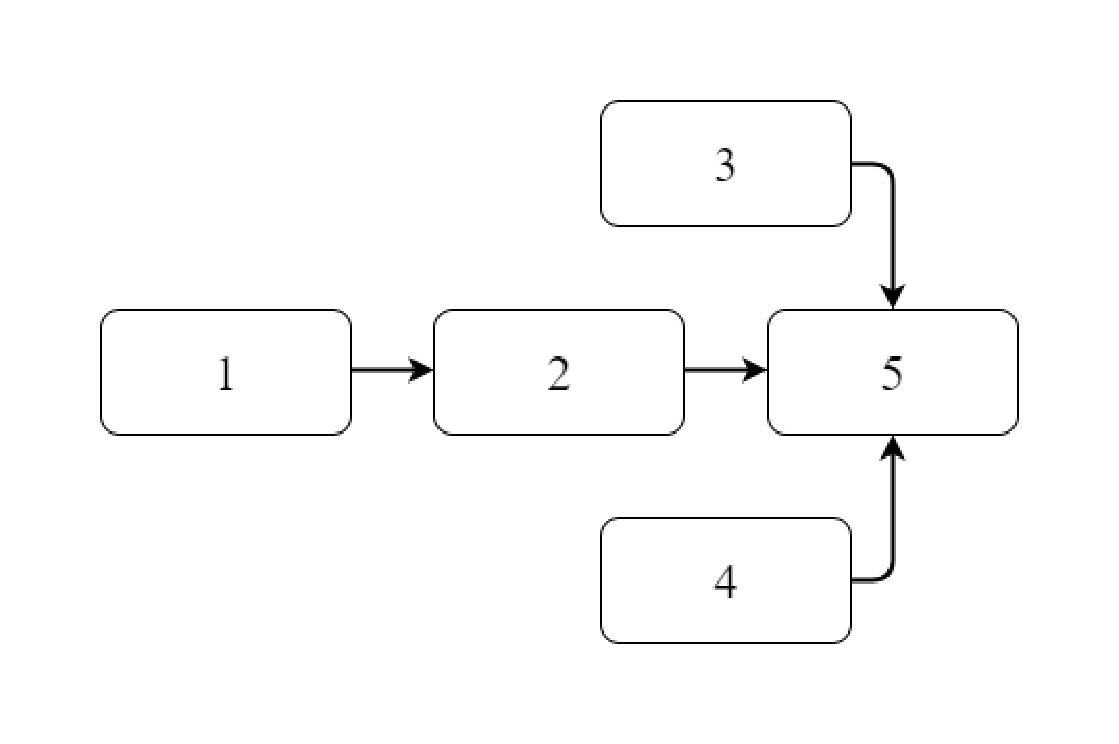
\includegraphics[width=1\linewidth]{3}}
					\label{pic:doubleInsertC}
				}
			\end{minipage}
			\hfill
			\begin{minipage}[h]{0.45\linewidth}
				\center \subfigure[]{
					{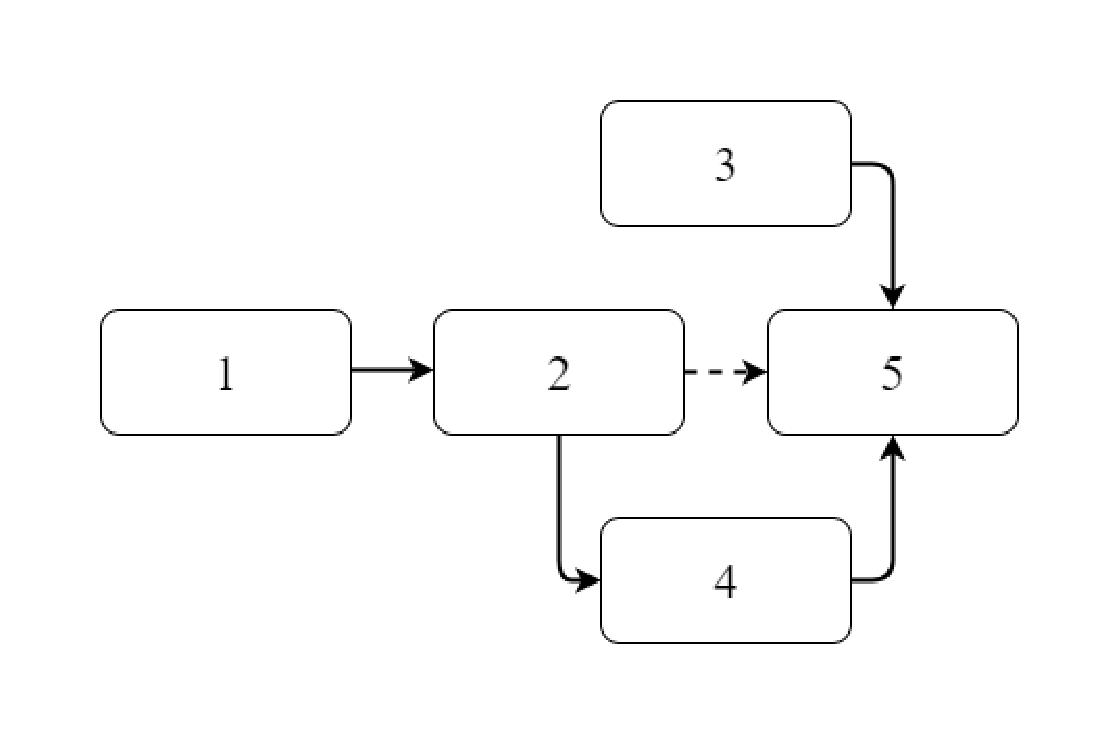
\includegraphics[width=1\linewidth]{4}}
					\label{pic:doubleInsertD}
				}
			\end{minipage}
			\begin{minipage}[h]{0.45\linewidth}
				\center \subfigure[]{
					{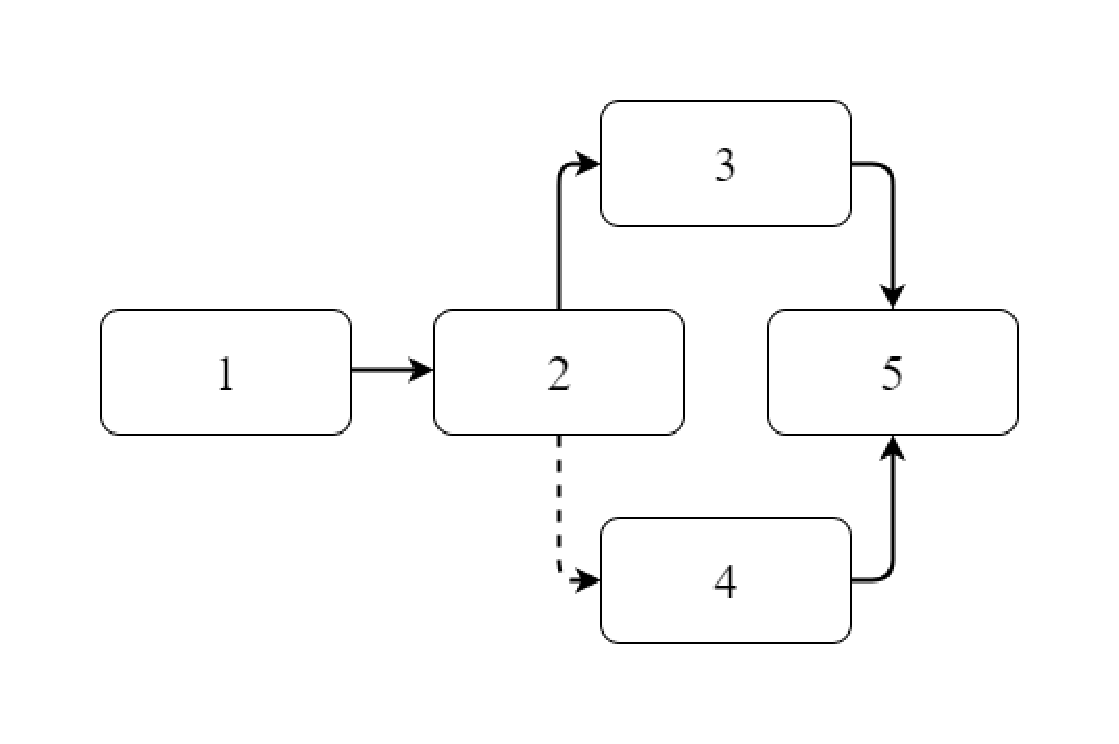
\includegraphics[width=1\linewidth]{5}}
					\label{pic:doubleInsertE}
				}
			\end{minipage}
			\caption{Одновременное добавление в 2 потоках: a) начальное состояние, b) А поставил ссылку на 5, c) Б поставил ссылку на 5, d) А сменил ссылку <<Next>> у 2, e) Б сменил ссылку <<Next>> у 2.}
		\end{figure}
		\par Реализация неблокирующего доступа использует типичный прием для неблокирующих алгоритмов - вечный цикл с операцией CAS и применение стратегии Back-off, описанной ранее. На каждом шаге цикла алгоритм пытается найти два элемента \textbf{а} и \textbf{б}, между которыми должен быть вставлен новый, и атомарно перезаписать ссылку <<Next>> с предыдущего элемента \textbf{(а)} на новый, при этом сравнивая, является ли эта ссылка до сих пор ссылкой на следующий \textbf{(б)}. Алгоритм выходит из цикла, когда попытка замены ссылки происходит успешно (Рис~\ref{pic:whileCas}). Такая реализация полностью решает вышеописанную проблему. При попытке перезаписать ссылку элемента \textbf{2} с \textbf{5} на \textbf{3}  (Рис~\ref{pic:doubleInsertE}), CAS завершается неудачей, потому что ссылка уже не на \textbf{5}, а на \textbf{4}. Алгоритм заново находит соседние элементы, и следующий уже не \textbf{5}, а \textbf{4}. На этом шаге цикла CAS уже выполняется успешно. Оба элемента вставлены правильно.
		\begin{figure}[h]
			\begin{lstlisting}
while (true)
{	
	1) (predsessor, subsessor) = FindPlace(newElement);
	2) newElement.Next = subsessor;
	2) if (CAS(ref predsessor.Next, newElement, subsessor));
		break
}
			\end{lstlisting}
			\caption{Шаг цикла. 1) находим соседние элементы, между которыми нужно вставить новый, 2) ссылку Next у нового элемента поместим на subsessor 3) пытаемся атомарно вставить}
			\label{pic:whileCas}
		\end{figure}
		\par Еще одна проблема может возникнуть при одновременным удалении и вставке двух последовательных элементов. Пусть есть список \textbf{1}-\textbf{2}-\textbf{4} (Рис~\ref{pic:insertDeleteA}). Поток \textbf{А} хочет добавить элемент \textbf{3}, поток \textbf{Б} удалить элемент \textbf{2}. Поток \textbf{Б} запоминает, что предыдущий элемент \textbf{1}, следующий \textbf{4}. Управление передается потоку \textbf{А}. Поток \textbf{А} вставляет элемент \textbf{3}, как это было описано ранее (Рис~\ref{pic:insertDeleteB}). Управление возвращается к потоку \textbf{Б}. Он атомарно заменяет ссылку <<Next>> у элемента \textbf{1} на элемент \textbf{4} (Рис~\ref{pic:insertDeleteC}). В итоге элемент \textbf{3} <<потерялся>>.
		\begin{figure}[h!]
			\begin{minipage}[h]{0.45\linewidth}
				\center  \subfigure[]{
					{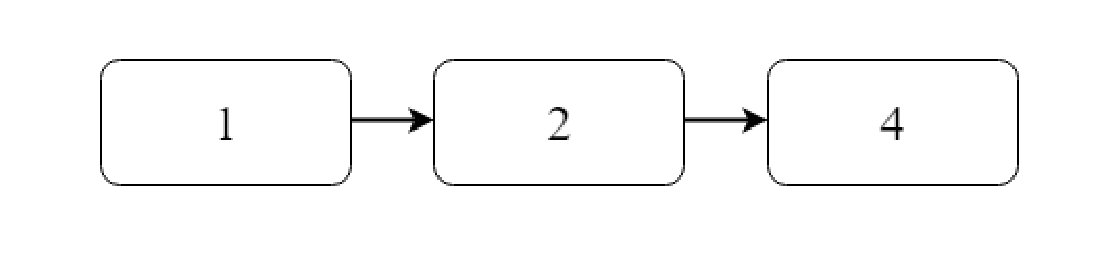
\includegraphics[width=1\linewidth]{6}}
					\label{pic:insertDeleteA}
				}
			\end{minipage}
			\hfill
			\begin{minipage}[h]{0.45\linewidth}
				\center \subfigure[]{
					{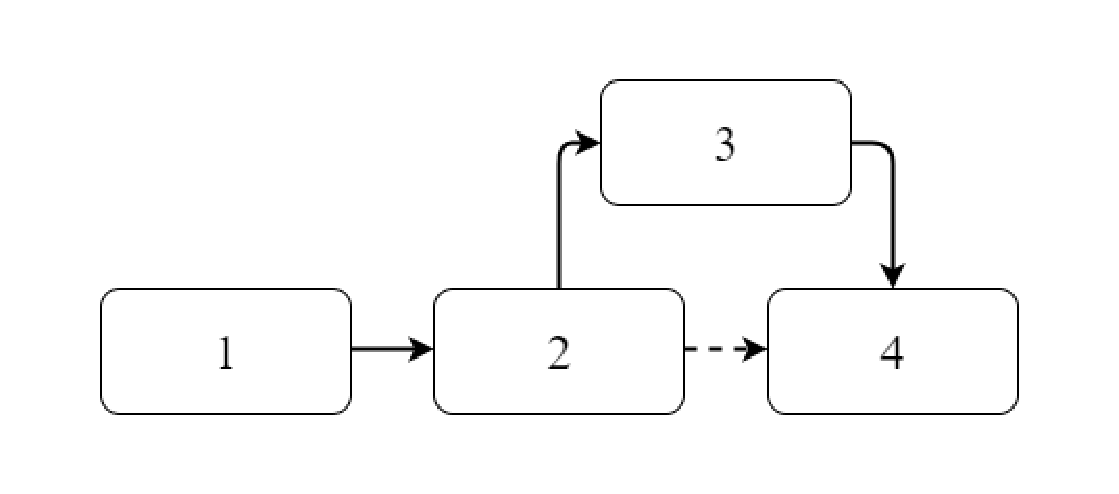
\includegraphics[width=1\linewidth]{7}}
					\label{pic:insertDeleteB}
				}
			\end{minipage}
			\vfill
			\begin{minipage}[h]{0.45\linewidth}
				\center \subfigure[]{
					{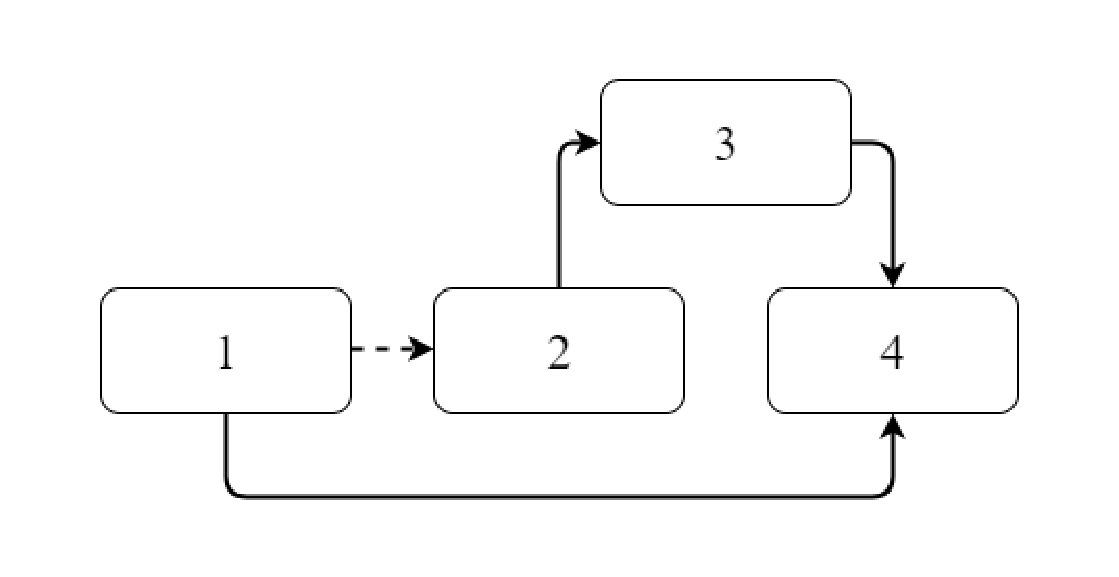
\includegraphics[width=1\linewidth]{8}}
					\label{pic:insertDeleteC}
				}
			\end{minipage}
			\caption{Одновременное добавление и удаление в 2 потоках: a) начальное состояние, b) А поставил ссылку на 4, c) Б сменил ссылку с 2 на 4.}
		\end{figure}
		\par Для устранения этой проблемы можно ввести дополнительный флаг в ссылку на объект (Рис~\ref{pic:listAMR}).
		\begin{figure}[h]
			\begin{lstlisting}
public class LinkedListNode<TElement>
{
	TElement Element;
	AtomicMarkableReference<LinkedListNode<TElement>, Flag> Next;
}
			\end{lstlisting}
			\caption{AtomicMarkableReference - структура, описанная в предыдущей главе, Flag может быть никаким или помеченным}
			\label{pic:listAMR}
		\end{figure}
		\par Теперь объект удаляется в два шага: 
		\begin{itemize}
			\item пометить как удаленный, но не удалить
			\item физически удалить. 
		\end{itemize}
		Можно заметить, что при помечивании ссылки на удаленный элемент, ситуация, изображенная на рисунке 5, существенно не изменится. Однако, при помечивании ссылки <<Next>> у удаляемого объекта, можно избежать потерь элементов. Теперь при вставке тройки из предыдущего примера ссылка <<Next>> у \textbf{2} уже будет помеченной. Это будет сообщать о том, что элемент в данный момент удаляется, а значит, манипулировать этой ссылкой пока что нельзя, надо заново перейти на новый виток в цикле и заново определить соседей. В итоге проблемы, описанной ранее при одновременной вставке и удалении не случится.
		\par Данный алгоритм в описанной ранее классификации является lock-free, так как один поток может помешать работе других потоков, но это будет значить, что он сам выполнил свою работу.
		\section{Улучшенный односвязный список}
		\par Вышеописанная реализация односвязного списка является неблокирующей, что, возможно, может ускорить работу программы, однако у нее до сих пор существует недостаток: если операции удаления происходят достаточно часто, то операции вставки будут также часто заканчиваться не успехом, из-за чего они каждый раз будут начинать сначала. В результате в худшем случае может получиться, что программа каждый раз заново пробегает весь список.
		\par Чтобы устранить эту проблему можно ввести еще две дополнительных абстракции. В ссылку <<Next>> добавить еще один флаг, который будет свидетельствовать, что следующий элемент в данный момент на стадии удаления. В сам элемент нужно добавить поле <<Backlink>>, который будет указывать на предыдущий элемент, который еще не участвует в удалении (Рис~\ref{pic:backlink}). 
		\begin{figure}[h]
			\begin{lstlisting}
public class LinkedListNode<TElement>
{
	TElement Element;
	LinkedListNode<TElement> Backlink;
	AtomicMarkableReference<LinkedListNode<TElement>, Flag> Next;
}
			\end{lstlisting}
			\caption{AtomicMarkableReference - структура, описанная в предыдущей главе, Flag может быть никаким, или помеченным на удаление, или помеченным на невозможность удаления}
			\label{pic:backlink}
		\end{figure}
		Теперь операция удаления будет проходить не в два, а в три этапа. Между двумя этапами из предыдущего алгоритма появится новый этап. Теперь после помечивания удаляемой вершины на удаление (Рис~\ref{pic:deleteA}) алгоритм добавляет в ссылку <<Next>> у предыдущей вершины новый флаг, который будет обозначать, что в данный момент вершина участвует в удалении, и ее саму удалять нельзя. У удаляемой вершины алгоритм устанавливает ссылку <<Backlink>> на ближайшую предыдущую вершину, которая еще не помечена новым флагом (Рис~\ref{pic:deleteB}). Теперь каждый раз, когда вставка не может завершиться успехом, поток будет по ссылкам <<Backlink>> возвращаться не в самое начало, а в первую вершину, следующая за которой еще не удаляется. Это позволяет еще немного ускорить работу программы, так как при каждой неудачной вставке, возможно, больше не нужно проходить лист полностью заново.
		\begin{figure}[h!]
			\begin{minipage}[h]{0.45\linewidth}
				\center \subfigure[]{
					{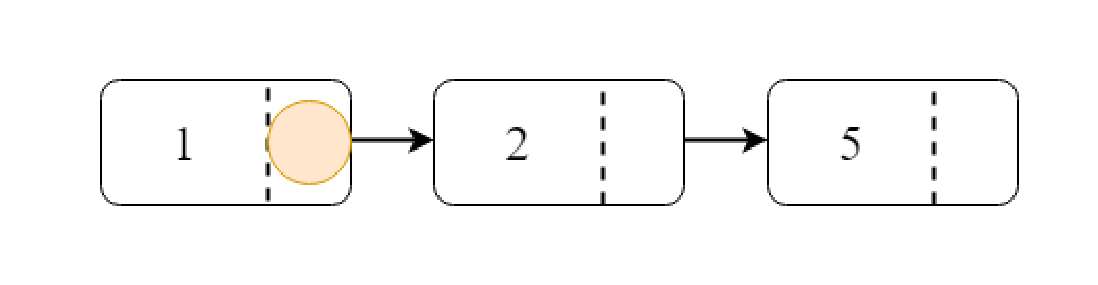
\includegraphics[width=1\linewidth]{9}}
					\label{pic:deleteA}
				}
			\end{minipage}
			\hfill
			\begin{minipage}[h]{0.45\linewidth}
				\center \subfigure[]{
					{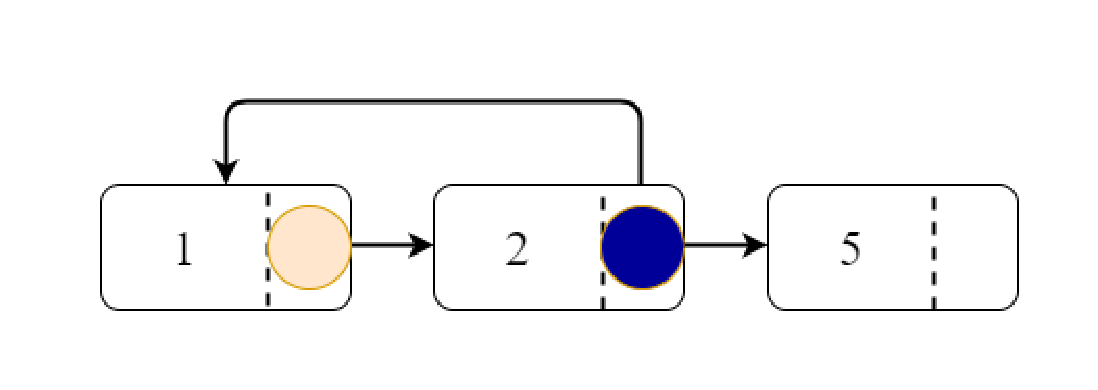
\includegraphics[width=1\linewidth]{10}}
					\label{pic:deleteB}
				}
			\end{minipage}
			\vfill
			\begin{minipage}[h]{0.45\linewidth}
				\center \subfigure[]{
					{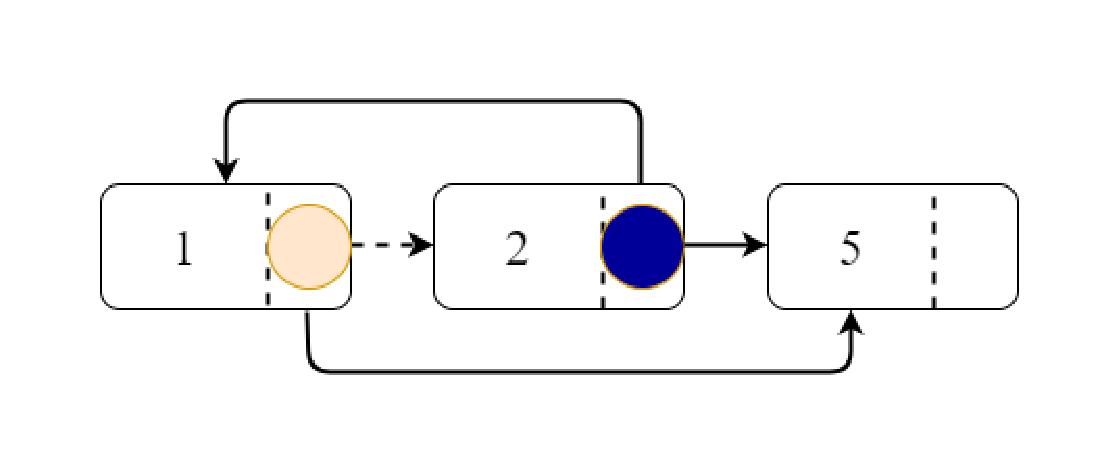
\includegraphics[width=1\linewidth]{11}}
					\label{pic:deleteC}
				}
			\end{minipage}
			\caption{Удаление в 3 этапа: a) помечивание на участие в удалении, b) помечивание на удаление, c) реальное удаление.}
		\end{figure}
		\section{Список с пропусками}
		\par Список с пропусками в своей структуре содержит несколько самосортирующихся односвязных списков. Поэтому алгоритм неблокирующего списка с пропусками будет использовать все те же идеи, что и неблокирующий односвязный список. Остается разобраться, как применить все те же идеи, но вставляя и удаляя не 1 элемент, а сразу столбец. 
		\par Вставка, как и в однопоточном варианте осуществляется снизу-вверх (Рис~\ref{pic:skiplist}). Однако, в данном случае на каждом уровне приходится искать заново, иначе можно запомнить элемент, который какой-то другой поток уже удалил.
		\begin{figure}[h!]
			\begin{minipage}[h]{0.45\linewidth}
				\center 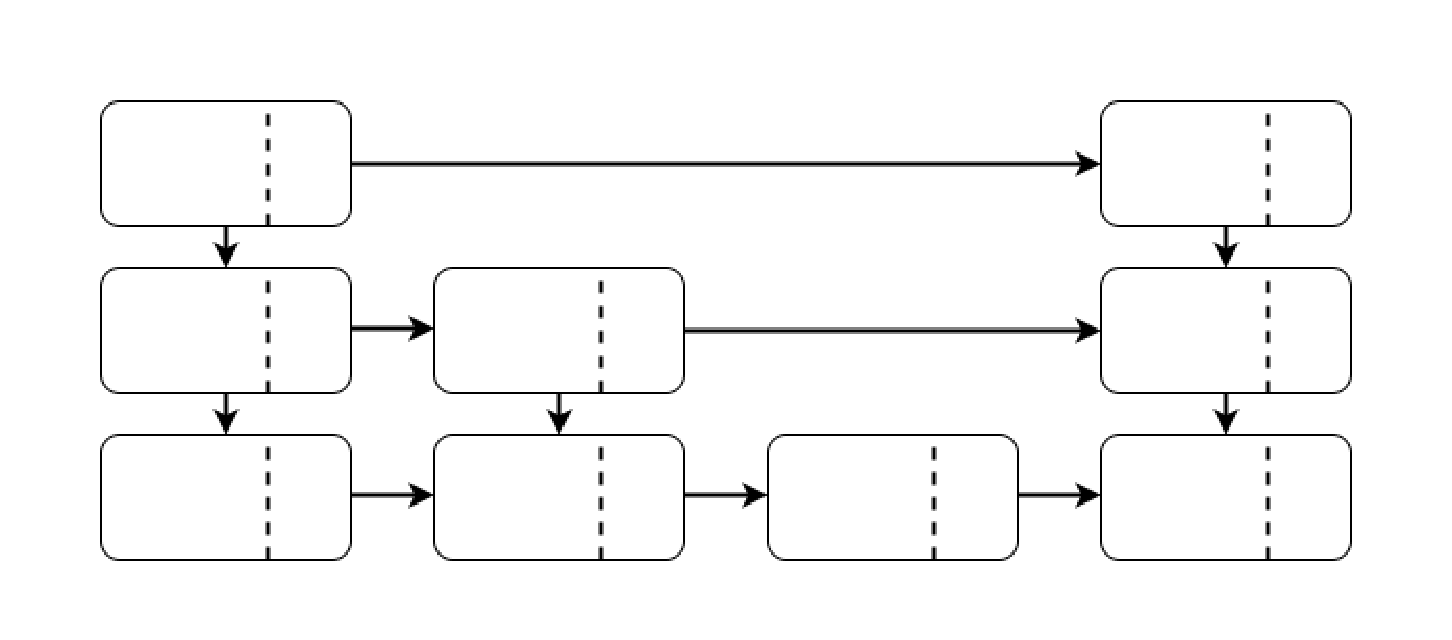
\includegraphics[width=1\linewidth]{12} a) \\
			\end{minipage}
			\hfill
			\begin{minipage}[h]{0.45\linewidth}
				\center 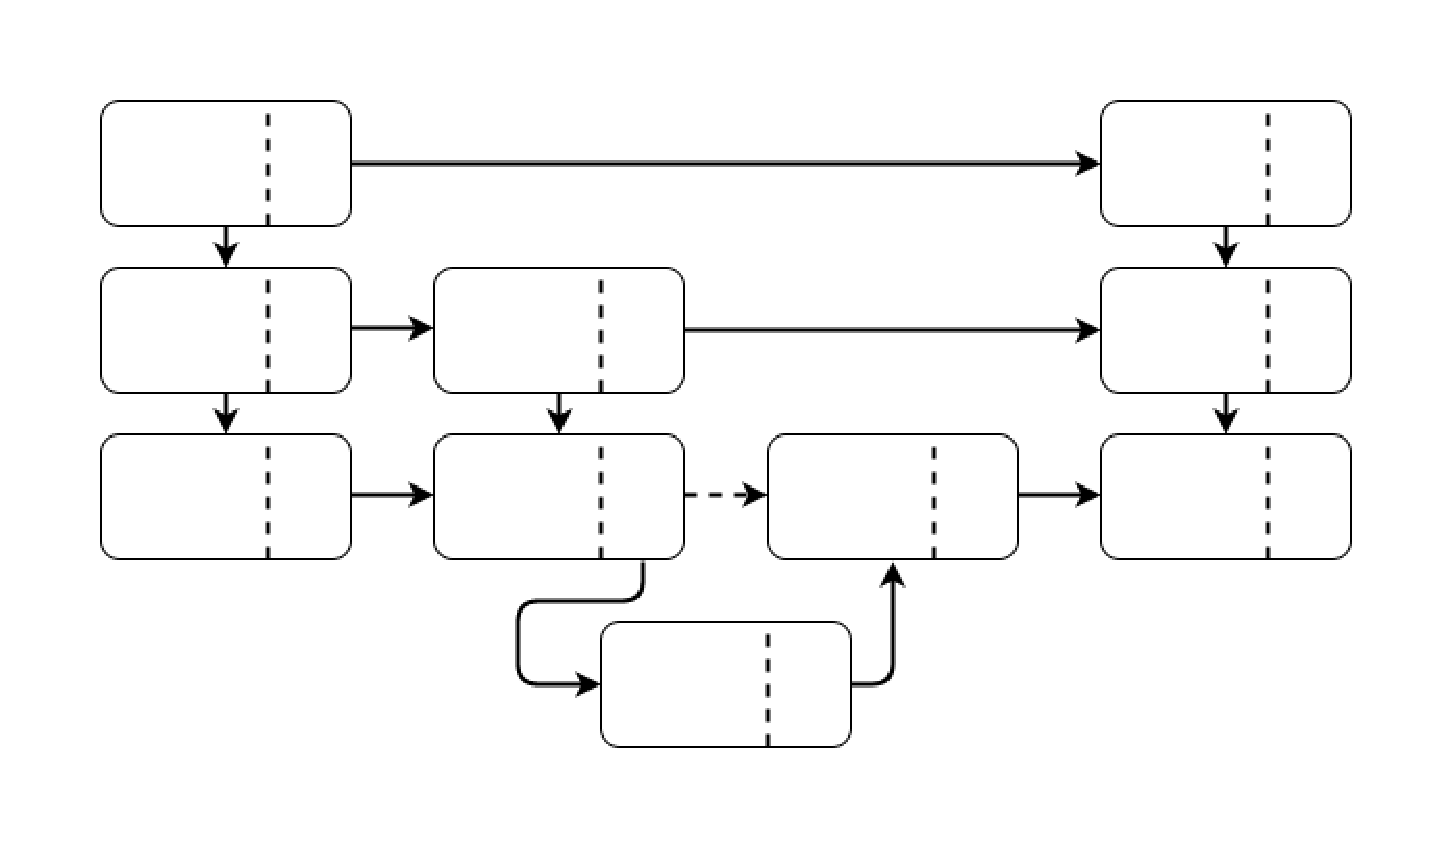
\includegraphics[width=1\linewidth]{13} b) \\
			\end{minipage}
			\vfill
			\begin{minipage}[h]{0.60\linewidth}
				\centering 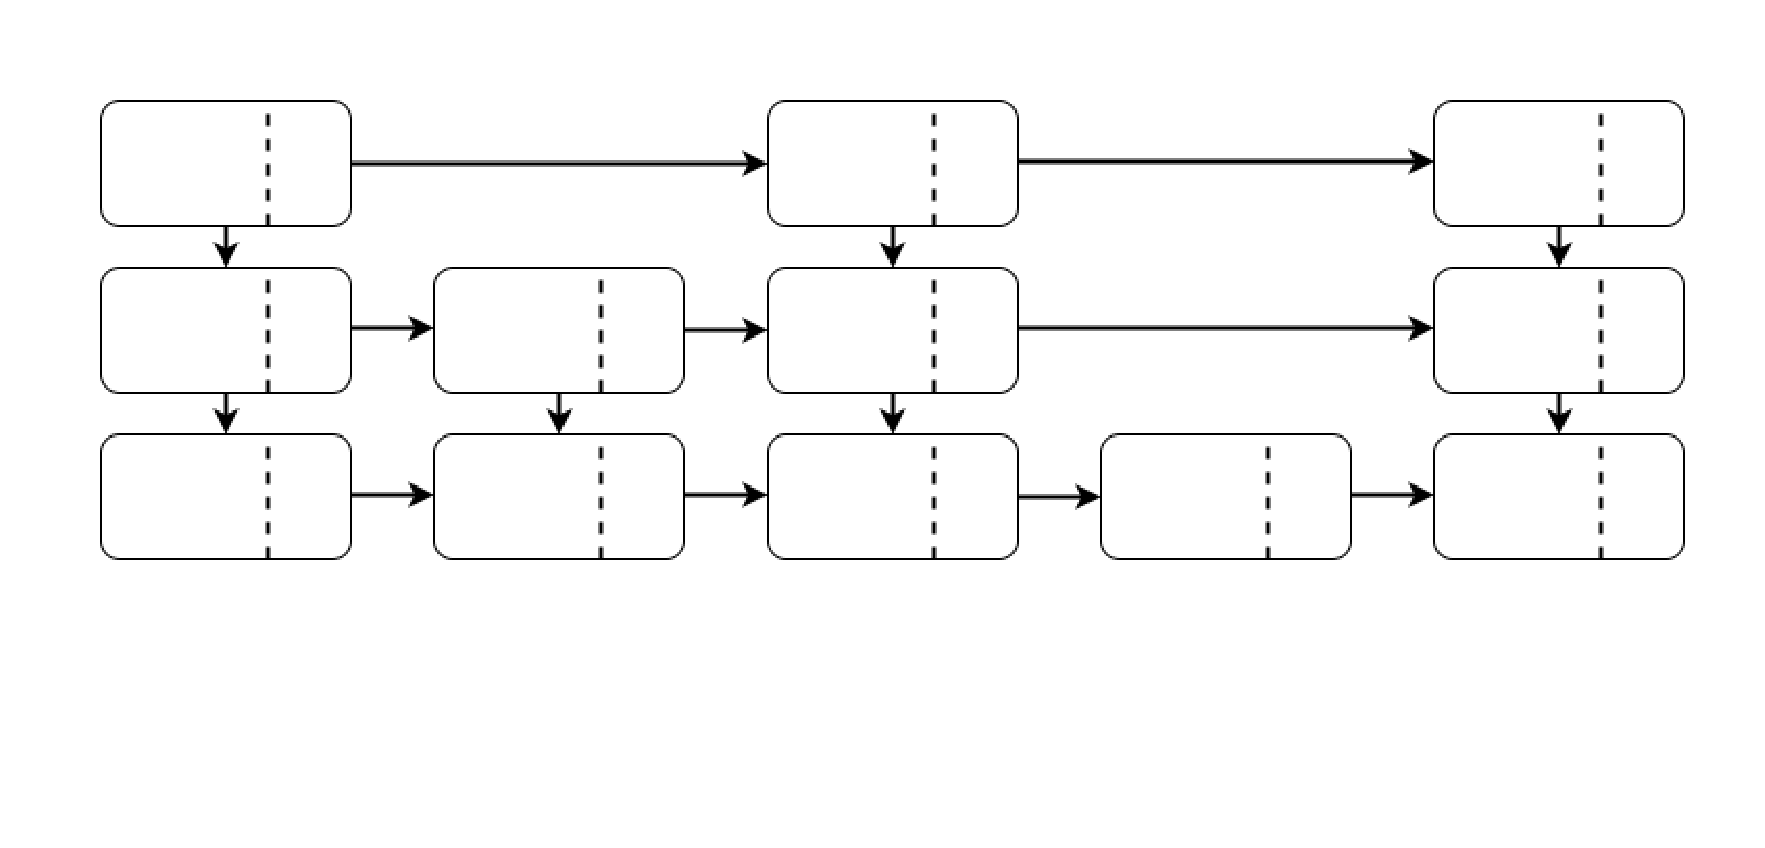
\includegraphics[width=1\linewidth]{14} c)\\
			\end{minipage}
			\caption{Добавление в список с пропусками: a) начальное состояние, b) добавление элемента на самом нижнем уровне, c) добавление остальных элементов.}
			\label{pic:skiplist}
		\end{figure}
		\par Удаление тоже происходит, начиная с удаления вершины на самом нижнем уровне. Этого действия достаточно, чтобы весь столбец считался удаленным. При каждом следующем поиске по списку нужно проверять не удалена ли текущая вершина, а удалена ли ее вершина с первого уровня (вершины реально не удаляются из памяти, но на них больше никто не ссылается, поэтому можно считать, что они больше не принадлежат к списку, так как они недостижимы). Если вершина с первого уровня удалена, то нужно удалить и текущую вершину, а также больше не ссылаться на нее и не строить из нее ссылки на новые вершины (Рис~\ref{pic:skiplistDelete}).
		\begin{figure}[h!]
			\begin{minipage}[h]{0.45\linewidth}
				\center 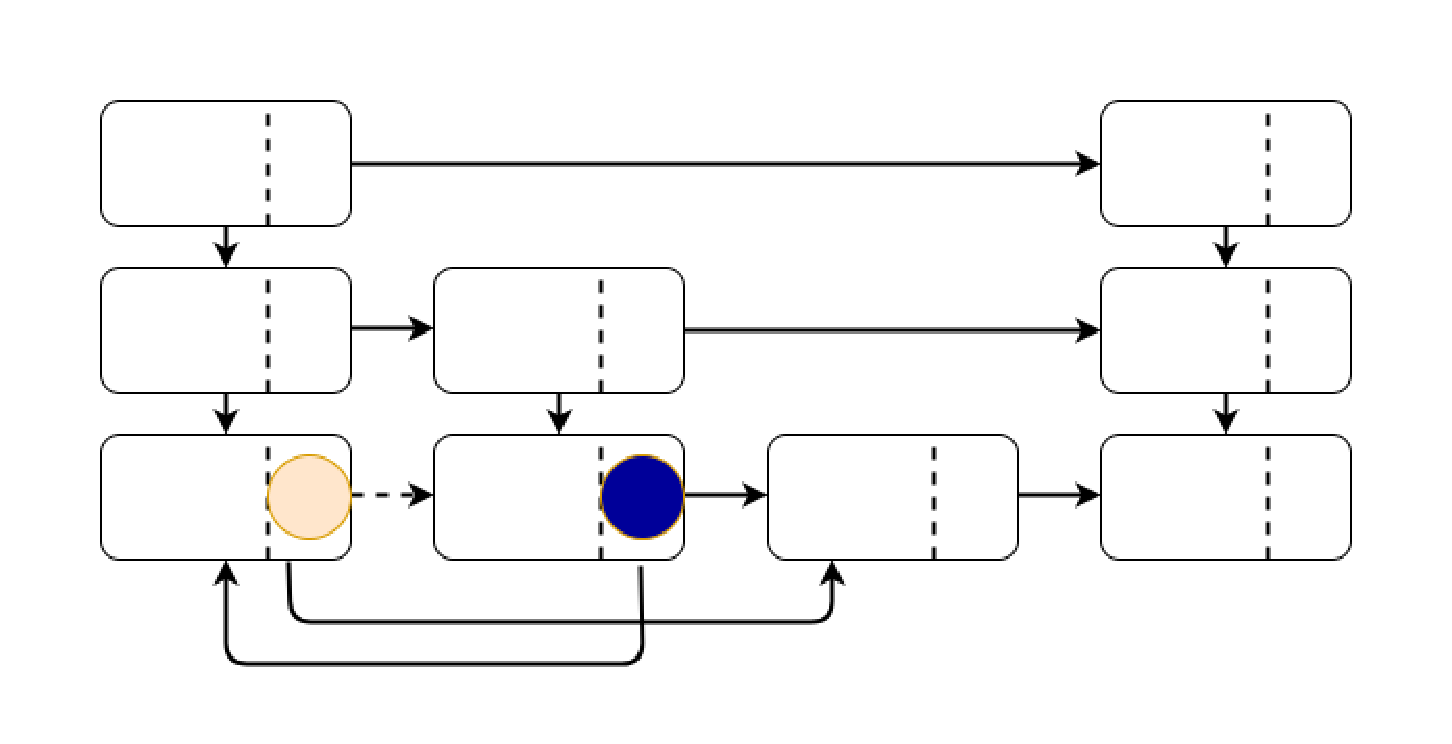
\includegraphics[width=1\linewidth]{15} a) \\
			\end{minipage}
			\hfill
			\begin{minipage}[h]{0.45\linewidth}
				\center 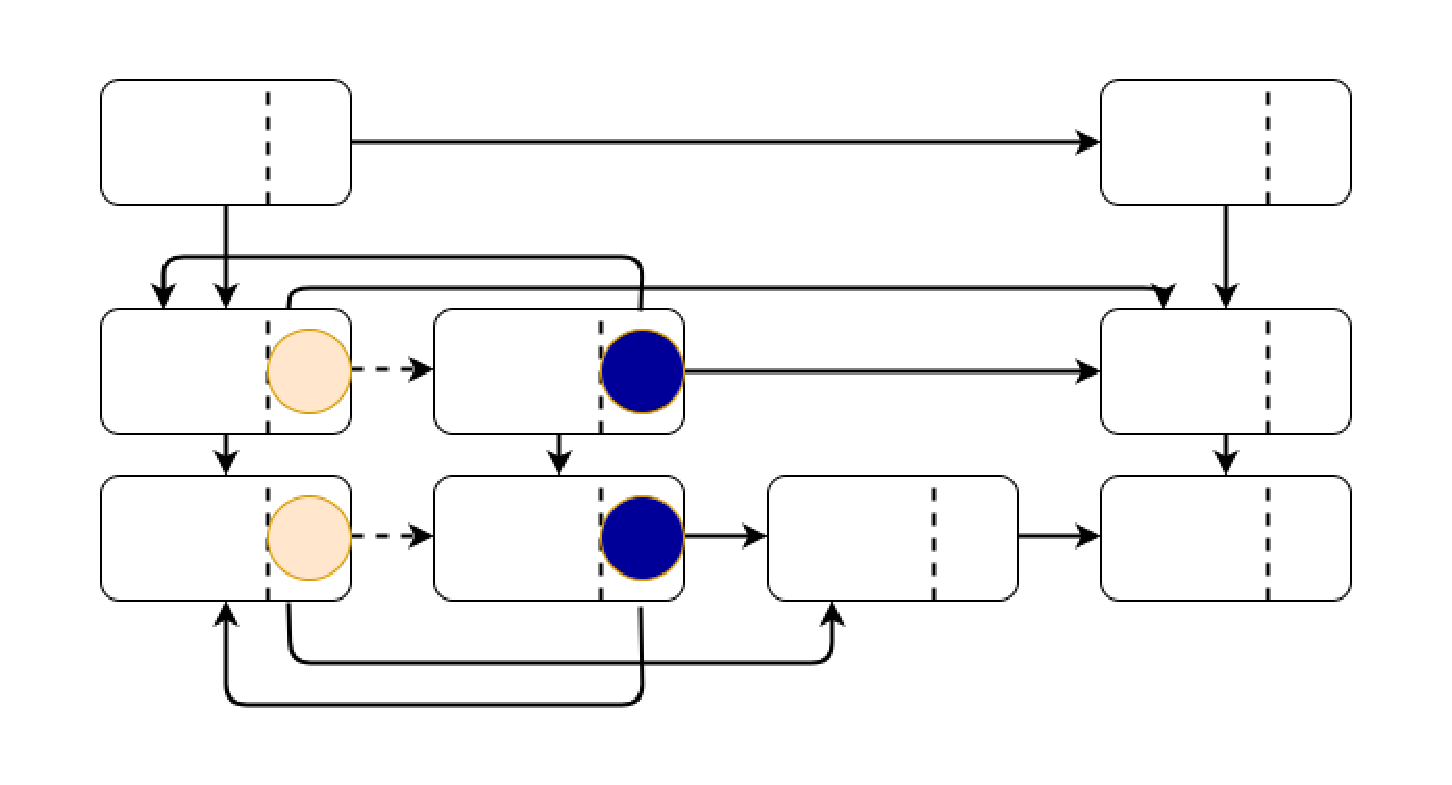
\includegraphics[width=1\linewidth]{16} b) \\
			\end{minipage}
			\vfill
			\begin{minipage}[h]{0.45\linewidth}
				\centering 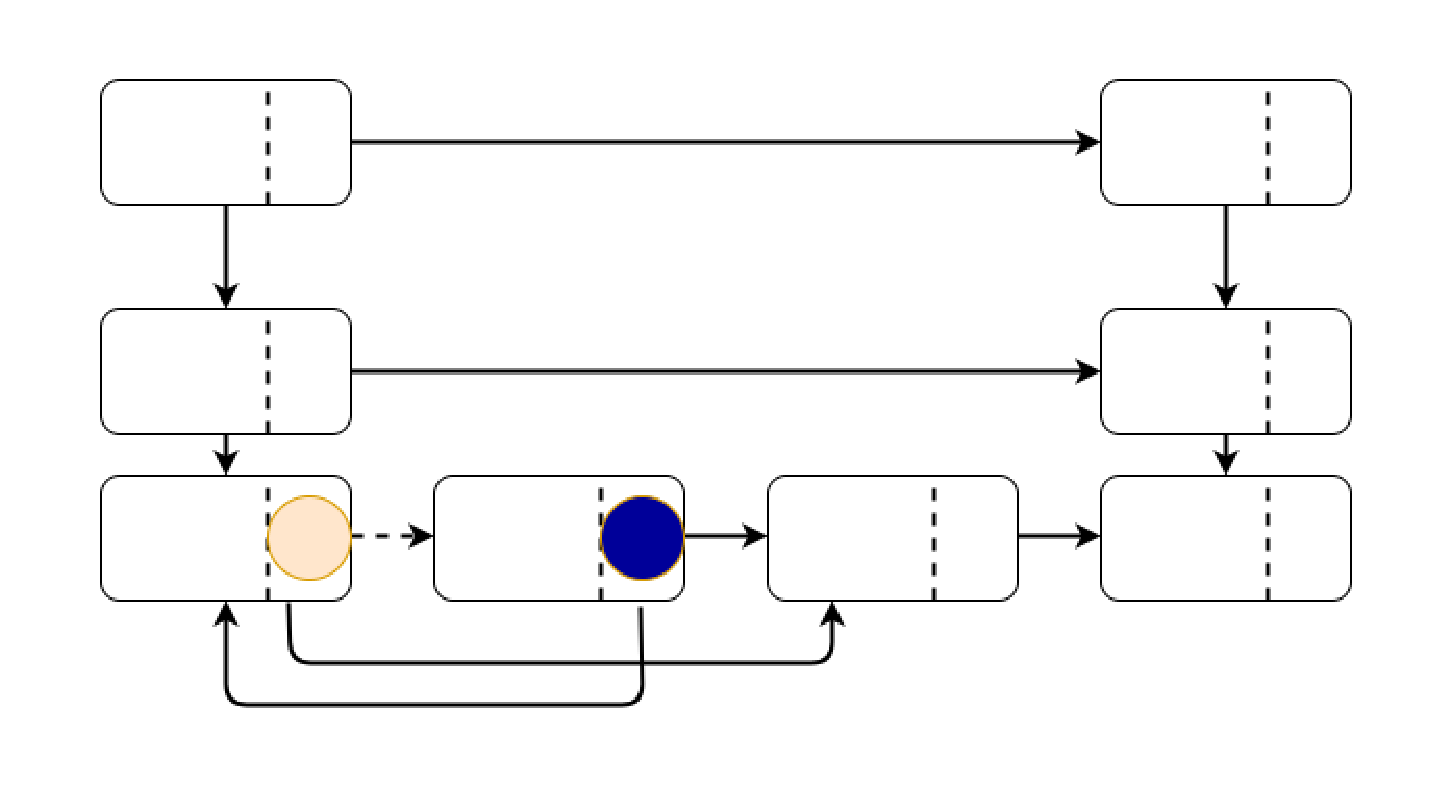
\includegraphics[width=1\linewidth]{17} c)\\
			\end{minipage}
			\hfill
			\begin{minipage}[h]{0.45\linewidth}
				\center 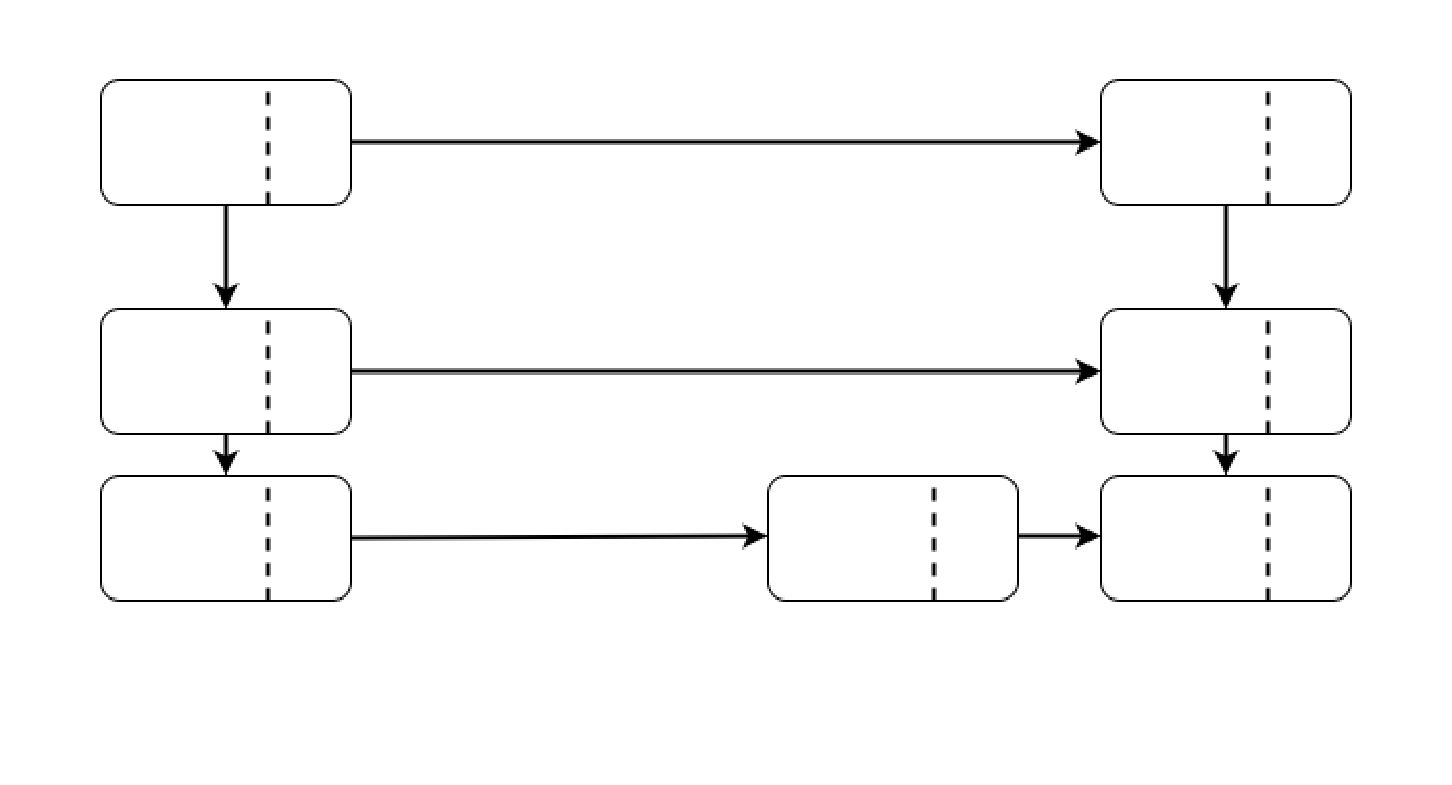
\includegraphics[width=1\linewidth]{18} d) \\
			\end{minipage}
			\caption{Удаление из списка с пропусками: a) логическое удаление вершины на нижнем уровне, b) логическое удаление вершин на остальных уровнях, c) физическое удаление вершин на уровнях, выше первого, d) физическое удаление вершины на первом уровне.}
			\label{pic:skiplistDelete}
		\end{figure}
		\par Списки внутри списка с пропусками можно также улучшить с помощью второго алгоритма односвязного списка.
		\par Так как список с пропусками основан на односвязных списках, то он тоже является lock-free.
		\section{Хеш-таблица}
		\par Хеш-таблица - структура данных, основыванная на массиве с произвольным доступом. На данный момент не придумано алгоритма, как можно реализовать строгий параллельный доступ к одной ячейке памяти на запись. Однако блокировать каждый раз весь массив, очевидно, неправильно. В таких случаях используют другой подход.
		\begin{figure}[h]
			\begin{minipage}[h]{1\linewidth}
				\center 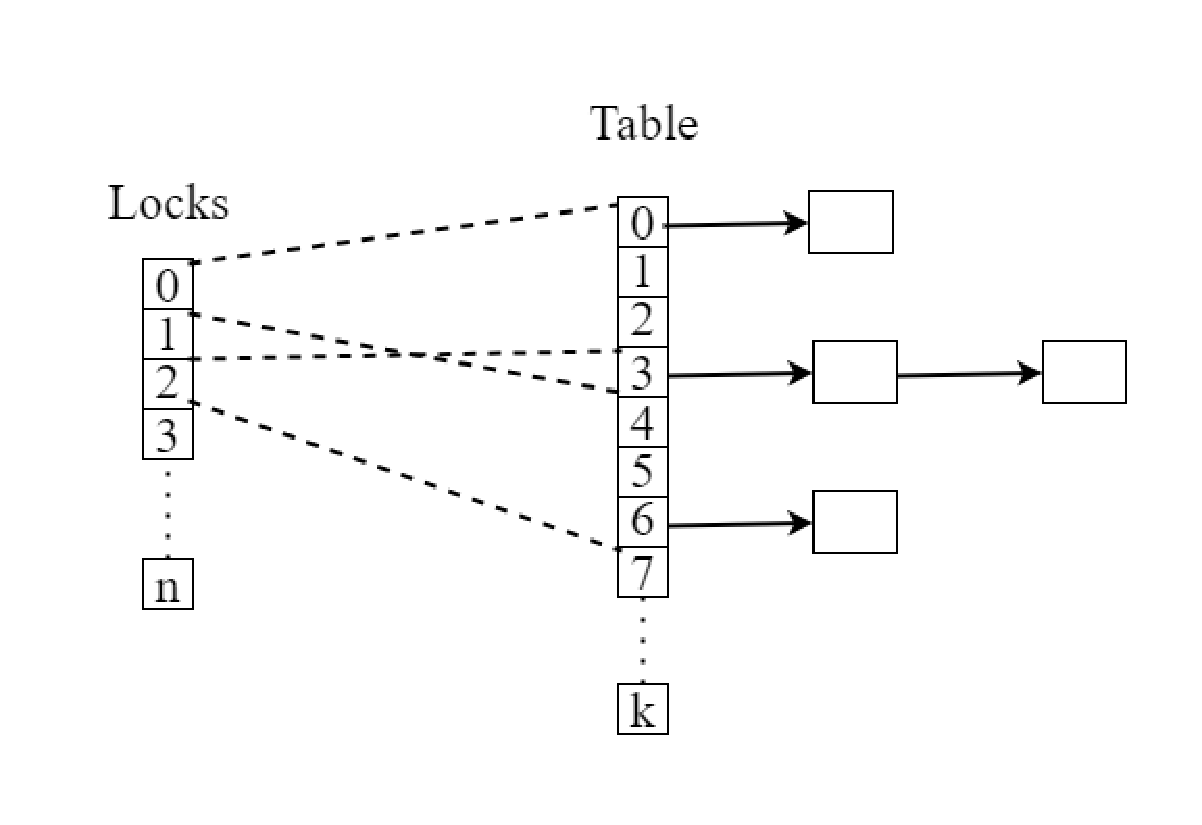
\includegraphics[width=1\linewidth]{19} \\
			\end{minipage}
			\caption{Хеш-таблица. Слева массив блокировок, справа сама хеш-таблица}
			\label{pic:hashTable}
		\end{figure}
		\par Весь массив разбивают на кусочки. Чаще всего используют куски одинаковой длины, распределяя их равномерно по массиву. Куски могут пересекаться или не пересекаться (Рис~\ref{pic:hashTable}). В технике striping имеется два массива — массив блокировок и хеш-таблица. Во время операции модификации высчитывается нужный хеш, находится место в массиве, где этот элемент должен быть изменен, и блокируется только тот кусок, которому принадлежит данный элемент. После модификации блокировка отпускается.
		\par При увеличении количества элементов количество кусков списки коллизий становятся очень большие и все преимущества хеш-таблиц становятся невозможными. Для расширения хеш-таблицы на весь массив в массиве блокировок захватывается блокировка, массив хеш-таблицы обновляется, после чего все блокировки освобождаются. Важно заметить, что массив блокировок остается неизменного размера, но с каждым увеличением массива хеш-таблицы длина каждого куска увеличивается.
		\par Такой подход не обеспечивает неблокирующего доступа, этот алгоритм хеш-таблицы является комбинацией неблокирующего и блокирующего алгоритмов. Так же он сильно зависит от длины массива блокировок. Если он слишком большой, то каждый его элемент покрывает очень маленький кусок в основном массиве, что близко к блокировке каждого элемента в основном массиве. Если он слишком маленький, то каждый его элемент покрывает слишком большой кусок в основном массиве, что близко к блокировке всего основного массива.
		
		\newpage
		
		\chapter{3. Тестирование}
		\section{Модульное тестирование}
		\par Тестирование параллельного алгоритма всегда трудно. Приходится каждый раз задумываться о том, как будут работать те или иные функциональности вместе. В данной работе использовано два основных подхода. Первый заключается в изолированном тестировании каждого метода в одном потоке. Тестирование параллельного кода всегда должно начинаться с проверки функциональности в однопоточном искусственно-созданном окружении. Далее проверяются простые сценарии в нескольких потоках, чтобы проверить, что они вообще корректно взаимодействуют между собой, т. е. делают то, что от них <<ожидают>> в каждом конкретном сценарии.
		\par Второй подход: <<тестирование грубой силой>>. В этом случае запускается большое количество потоков или выполняется большое количество операций одновременно. При увеличении числа операций вероятность ошибки увеличивается, в этом и заключается данный метод. Однако даже это не гарантирует, что программа работает правильно. В некоторых случаях сценарии неправильной работы кода настолько редки, что можно вообще никогда их не получить ошибку в тестировании.
		\par Отсюда плавно вытекает третий подход: тестирование аналитически. Он заключается в тщательном продумывании всех возможных сценариев, проверки каждой строчки кода, попытки смоделировать выполнение программы и найти потенциальные ошибки. Однако большая проблема данного подхода: <<человеческий фактор>>. Иногда такую проверку все же можно сделать формально и наглядно. В данной статье в ссылках на алгоритмы приведен подробный анализ корректности работы алгоритма, заключающийся в разборе всех возможных сценариев.
		\section{Тестирование производительности}
		\par Если тестирование работоспособности алгоритма нужно для проверки, что алгоритм работает корректно, то оценка производительности нужна для представления, реализуем ли этот алгоритм на практике. Проверяется, соответствует ли время работы или количество используемой памяти теоретическим оценкам. Чаще всего такое тестирование проходит в сравнении с эталоном. В данной работе эталоном представлялся дополнительный алгоритм, основанный на блокировании структуры. Ожидается, что на большом количестве потоков, этот алгоритм будет работать в среднем хуже, чем неблокирующий алгоритм.
		\par Для оценки производительности можно использовать различные метрики. В данной работе рассматривалось несколько различных тестовых окружений, в каждом из которых все реализованные структуры данных и варианты работы в 1, 2 и 8 потоках. 
		\par В качестве тестового окружения был выбран компьютер Intel Core i7-4790 CPU 3.60GHz (Haswell), ProcessorCount=8 Frequency=3507505 Hz,  Resolution=285.1029 ns, Timer=TSC. Операционная система: Windows 10. C\# Clr 4.0.30319.42000, 64bit LegacyJIT/clrjit-v4.6.127.1;compatjit-v4.6.1055.0.
		В качестве тестовых сценариев были выбраны: 
		\begin{itemize}
			\item вставка, удаление, поиск по-отдельности
			\item только вставка и поиск в соотношении 9:1
			\item вставка, поиск и удаление в соотношении 2:7:1			
		\end{itemize}
		\section{Результаты}
		\par Полные результаты представлены по ссылке \cite{My}.
		\par Из результатов можно отметить, что неблокирующие структуры данных, действительно, с ростом количества потоков и числа обрабатываемых элементов часто работают лучше, чем блокирующие аналоги. Например, поиск в 8 потоках 100000 элементов неблокирующая хеш-таблица осуществляет за 2,894.9 мксек., а блокирующая за 5,222.1 мксек., добавление и поиск 10000 элементов в блокирующей реализации односвязного списка осуществляется за 625.1 мксек., а в блокирующем за 656.7 мксек.
		\par Также можно привести некоторые рекомендации использования. Если чаще всего происходит операция проверки на принадлежность, то быстрее всего в среднем работает хеш-таблица, как и в неблокирующей реализации. Хуже всего поиск осуществляется в односвязном списке, опять как в неблокирующей реализации. При частой вставке элементов лучше всего работает односвязный список, так как он меньше всего задействует вспомогательных элементов структуры. Хуже всего работает хеш-таблица. При частых операциях лучше всего работает хеш-таблица, потому что при малых коллизиях очень редко приходится синхронизировать параллельные потоки. Если вставка и поиск происходят примерно в пропорциях 1:9, то список с пропусками и односвязный список справляются примерно одинаково, хеш-таблица тоже незначительно проигрывает. А вот при вставке, поиске и удалении в соотношении 2:7:1 неожиданно выигрывает односвязный список, однако все остальные структуры данных осуществляют эти операции за такой же порядок времени.				
		
		\newpage
		
		\chapter*{Заключение}
		\addcontentsline{toc}{chapter}{Заключение}
		\par Результатом данной работы является готовый протестированный модуль с реализованными потокобезопасными неблокирующими структурами данных. Были выбраны алгоритмы, способные реализовать интерфейс set и адаптированы под язык с управляемой памятью. Также были произведены тысты производительности, которые показали практическую применимость выбранных алгоритмов.
		
		\addcontentsline{toc}{chapter}{Список литературы}
		\bibliographystyle{utf8gost705u}
		\bibliography{biblio}  
		
		\newpage
	}
	
\end{document}